% LaTeX Template for short student reports.
% Citations should be in bibtex format and go in references.bib
\documentclass[a4paper, 12pt]{article}
\usepackage[top=2cm, bottom=3cm, left = 2cm, right = 2cm]{geometry} 
\geometry{a4paper} 
\usepackage[utf8]{inputenc}
\usepackage{textcomp}
\usepackage{graphicx} 
\usepackage{amsmath,amssymb}  
\usepackage{bm}  
\usepackage{memhfixc} 
\usepackage{fancyhdr}
\usepackage{float}
\usepackage{booktabs}
\usepackage{listings}
\usepackage{xcolor}
\usepackage{xepersian}
\lstset{escapeinside={<@}{@>}}
\settextfont[Scale=1.]{HM FNazli}
\setlatintextfont[Scale=.9]{Noto Sans}
\pagestyle{fancy}

\title{\lr{JOS IPC Implementation}}
\author{
    علی کریمی \and
    حسین افکار \and
    محمدرضا ولی
    }
%\date{}

\begin{document}
\maketitle
\section{
    مقدمه و پیش‌نیاز‌ها
}
در تمرین شماره چهار ما باید قابلیت ارتباط میان پردازه‌ای را به کرنل
\lr{JOS}
اضافه کنیم.
کرنلی که در تمرین قبل در اختیار ما قرار گرفته است کاستی‌هایی دارد که باید برطرف کنیم.
این کاستی‌ها عبارت‌اند از
\begin{itemize}
    \item مدیریت حافظه مجازی
    \item ساختن پردازه
    \item \lr{Trap Handler}
    \item زمان‌بند
    \item فراخوانی سیستمی 
    \lr{Fork}
\end{itemize}
برای این‌کار ابتدا می‌توانیم به سورس
\lr{JOS}
در دانشگاه
\lr{MIT}
مراجعه کنیم.
در این سورس موارد فوق وجود دارند که ما می‌توانیم فراخوانی‌های مورد نیاز را از آن‌ها کپی کنیم.
مدیریت حافظه مجازی در فایل‌های
\lr{\textit{pmap.c, pmap.h}}
قرار دارند.
برای اینکه بازه‌های حافظه‌ای قابل استفاده از بایوس دریافت شوند این کد از یک روش عجیب استفاده می‌کند
که در آن با استفاده از ساعت بی‌درنگ سیستم محتویات
\lr{nvram}
بایوس خوانده می‌شوند.
به طور معمول در سیستم‌عامل‌های عادی از وقفه شماره ۱۵ استفاده می‌شود که برای این‌کار ما باید
به
\lr{real-mode}
برویم و سپس از آن برگردیم.
به خاطر اینکه
\lr{memory layout}
در نظر گرفته شده برای این سیستم‌عامل به حد کافی پیچیده است ما سعی نکردیم که
\lr{trampoline}
بین
\lr{real-mode}
و
\lr{protected-mode}
را پیاده‌سازی کنیم و به روش خواندن از ساعت بی‌درنگ بسنده کردیم. \\
بعد از اینکه حافظه مجازی ساخته شد باید سراغ ساختن محیط برای پردازه‌های سطح یوزر برویم
برای این کار لازم است که
\lr{trap}
ها را نیز پیاده‌سازی کنیم تا بتوانیم به وقفه‌ها و عملیات سیستمی در حین اجرای پردازه‌های سطح‌ کاربر پاسخ
بدهیم.
\lr{trap}
ها در فایل
\lr{\textit{trap.c, trap.h}}
پیاده‌سازی شده‌اند.
این کد ارتباط زیادی با بخش
\lr{multi processor}
و
\lr{scheduler}
دارد که نیاز پیاده‌سازی آن را توجیه می‌کند. همچنین خوب است که هنگام کدنویسی
\lr{IPC}
به آن‌ها دسترسی داشته باشیم چون که محل خطا‌ها را به ما نشان می‌دهند.
در ادامه باید محیط اجرای برنامه‌های یوزر پیاده‌سازی شود.
برای این‌کار باید فایل
\lr{elf}
توسط سیستم‌عامل پارس شده و محتویات
\lr{.text}
،
\lr{.data}
،و 
\lr{.bss}
در حافظه مجازی نشانده شوند.
فایل
\lr{elf}
در ویو
\lr{executable}
خود به ما می‌گوید که چگونه این کار را انجام دهیم.
به این صورت که بازه‌هایی را برای
\lr{LOAD}
به ما در
\lr{Program Header}
معرفی می‌کند و 
\lr{PC}
شروع برنامه نیز در
\lr{file header}
فایل
lr{elf}
قرار گرفته شده است.
\begin{figure}[H]
    \centering
    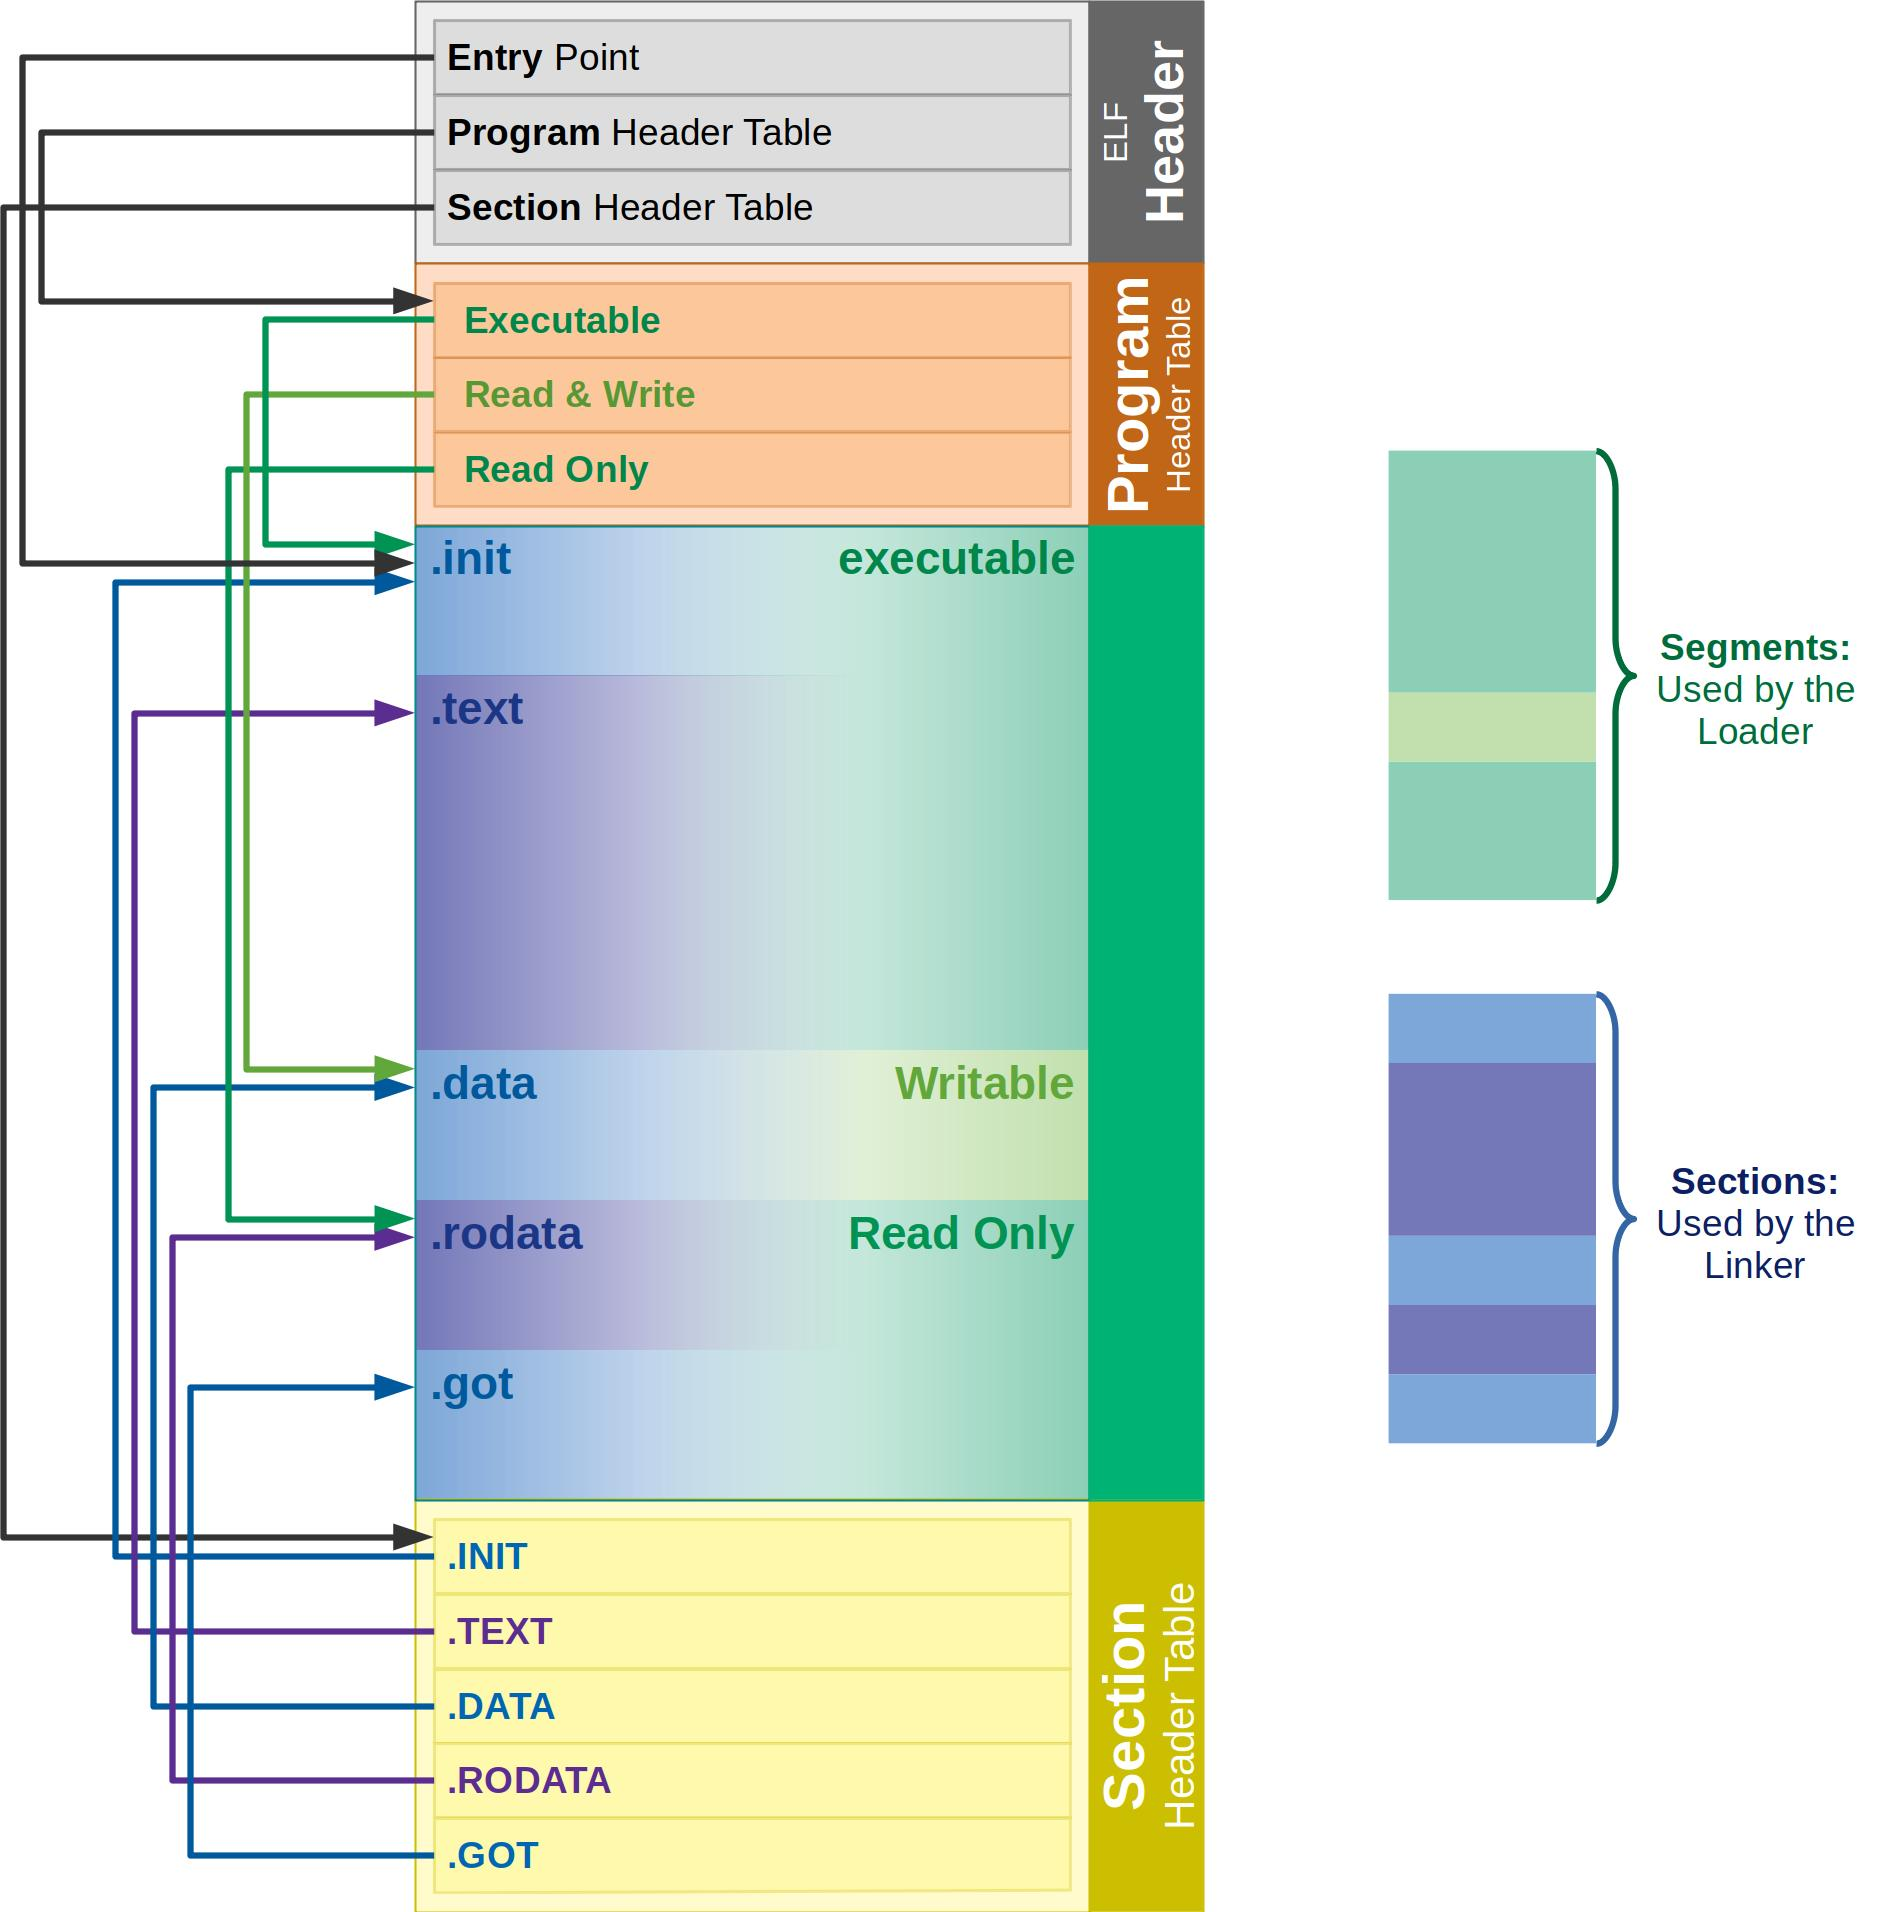
\includegraphics[width=0.6\textwidth]{typical_elf.jpg}
    \caption{
        نمونه ساختار یک فایل
        \lr{elf}
    }
    \label{fig1:output}
\end{figure}
در فایل‌های
\lr{\textit{env.c, env.h}}
یک محیط برای اجرای نرم‌افزار‌های سطح کاربر در نظر گرفته می‌شود که این محیط
ابتدا
\lr{Global Descriptor Table}
را در پردازنده‌های
\lr{Intel}
ست می‌کند و سپس آرایه‌ای برای نرم‌افزار‌های قابل اجرا در نظر گرفته می شود.
همچنین مسائل مربوط به
\lr{context switch}
و قرار دادن آدرس
\lr{Page Descriptor Table}
در رجیستر
\lr{cr3}
نیز از سمت این بخش سیستم‌عامل انجام می‌گیرد. \\
در ادامه لازم است که زمان‌بند پیاده‌سازی شود.
زمان بند روش
\lr{Round Robin}
را در پیش می‌گیرد و تابع
\lr{\textit{sched\_yield}}
را در اختیار ما می‌گزارد که برای پیاده‌سازی
\lr{IPC}
حدودا ضروری است.
در آخر فراخوانی سیستمی
\lr{Fork}
باید پیاده‌سازی گردد که این فراخوانی سیستمی
کل ایمیج پردازه را به صورت
\lr{Copy on Write}
کپی کرده و
\lr{Page Fault Handler}
پردازه را هم به همین دلیل عوض می‌کند.
در حین پیاده‌سازی این فراخوانی سیستمی به دلیل تنظیمات کامپایلر به خطای
\lr{Invalid Opcode}
برخورد کردیم که با استفاده از اطلاعاتی که 
\lr{trap handler}
به ما داد متوجه شدیم این خطا به دلیل استفاده کامپایلر از دستورات
\lr{SSE}
رخ می‌دهد.
بنابراین بین دو گزینه تنظیم مجازی‌ساز
\lr{QEMU}
و تنظیمات کامپایلر تنظیمات کامپایلر را انتخاب کردیم که با اضافه کردن گزینه
\lr{-mno-sse}
به
\lr{CFLAGS}
های تعریف شده در
\lr{GNUMakefile}
مورد برطرف شد که این اتفاق به ما نشان داد که چقدر هندل کردن
\lr{trap}
ها در مراحل اولیه طراحی سیستم‌عامل مهم است.
اتفاقات بسیار دیگری نیز در این سیستم‌عامل و روند نیز وجود دارند ولی به خاطر اینکه به پیاده‌سازی
\lr{IPC}
ما کم ربط هستند در مورد آن‌ها توضیحی داده نشده است.
در آخر عکسی از اجرای این سیستم‌عامل آورده شده است.
\begin{figure}[H]
    \centering
    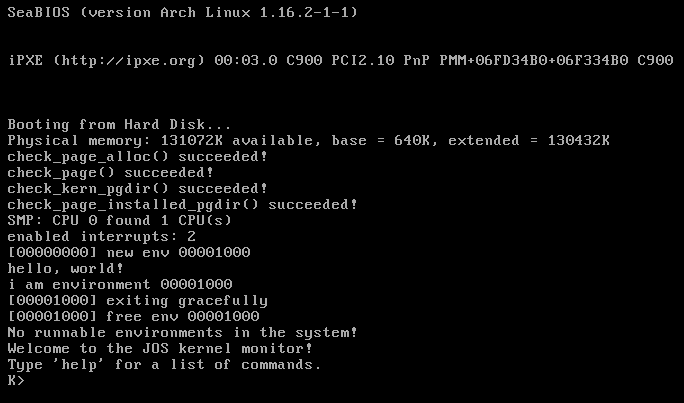
\includegraphics[width=1.0\textwidth]{hello.png}
    \caption{
        اجرای سیستم‌عامل به یک برنامه سطح کاربر که عبارتی را چاپ می‌کند.
    }
    \label{fig2:output}
\end{figure}
\section{
    پیاده‌سازی
    \lr{IPC}
}
در این بخش به الزامات پیاده‌سازی ارتباط میان‌ پردازه‌ای در این سیستم‌عامل می‌پردازیم.
در ابتدا نیاز است که دو فراخوانی سیستم
\lr{sys\_ipc\_try\_send}
و
\lr{sys\_ipc\_recv}
را بررسی کنیم.
فراخوانی اول به ما کمک می‌کند که با داشتن
\lr{envid}
از پردازه مورد نظر پیغام را به آن ارسال کنیم.
ولی این ارسال پیغام ممکن است همیشه موفق نباشد.
ارسال پیغام در این فراخوان سیستمی به این صورت است که یک پیج از حافظه و یک مقدار به پردازه دیگر ارسال می‌شوند.
و پردازه دیگر در صورتی که در وضعیت دریافت پیام باشد از این وضعیت در آمده و به وضعیت قابل اجرا
برای زمان‌بند برمی‌گردد. \\
فراخوانی شماره دو منتظر دریافت پیام می‌ماند و پردازه را در حالت منتظر برای دریافت قرار می‌دهد
و می‌خوابد. در صورتی که ما بخواهیم پیغامی را به پردازه‌ای بفرستیم که خودش را در حالت دریافت قرار
نداده باشد فراخوانی اول به ما مقدار
\lr{-1}
را بر می‌گرداند که به ما می‌گوید دوباره باید این فراخوانی را اجرا کنیم.
متن این فراخوانی‌ها در فایل‌
\lr{syscall.c}
آورده شده‌اند.
لازم است برای اینکه از این فراخوانی‌ها به درستی استفاده شود آن‌ها را به صورت کتاب‌خانه در اختیار
برنامه‌های سطح کاربر قرار می‌دهد.
این کار در فایل
\lr{\textit{lib/ipc.c}}
انجام شده است
\begin{figure}[H]
    \centering
    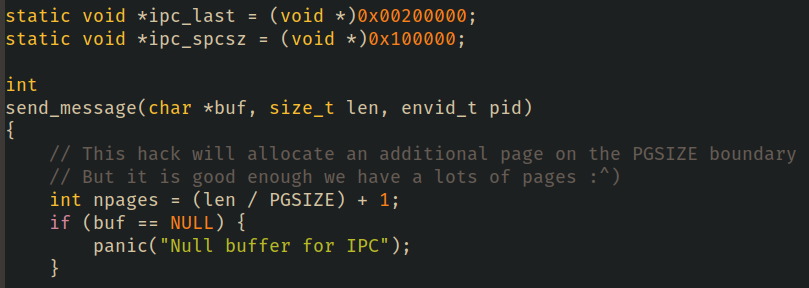
\includegraphics[width=1.0\textwidth]{send1.png}
    \caption{
        متن تابع
        \lr{send\_message}
    }
    \label{fig3:output}
\end{figure}
تابع
\lr{send\_message}
با متغیر‌های خواسته شده در صورت تمرین پیاده‌سازی شده است.
برای این کار ابتدا باید محیطی از حافظه را برای ارتباط میان‌ پردازه‌ای در نظر بگیریم.
با استناد به فایل
\lr{textit{memlayout.h}}
محل
\lr{0x00200000}
را برای این کار در نظر گرفتیم این محل توسط هیچ بخشی از سیستم استفاده نشده است.
ابتدا باید تعداد صفحات مورد نیاز برای دریافت را حساب کنیم.
این کار را با تقسیم کردن طول بافر بر سایز صفحه مجازی انجام می‌دهیم.
سپس در صورت ارسال بافر خالی
\lr{panic}
می‌کنیم.
\begin{figure}[H]
    \centering
    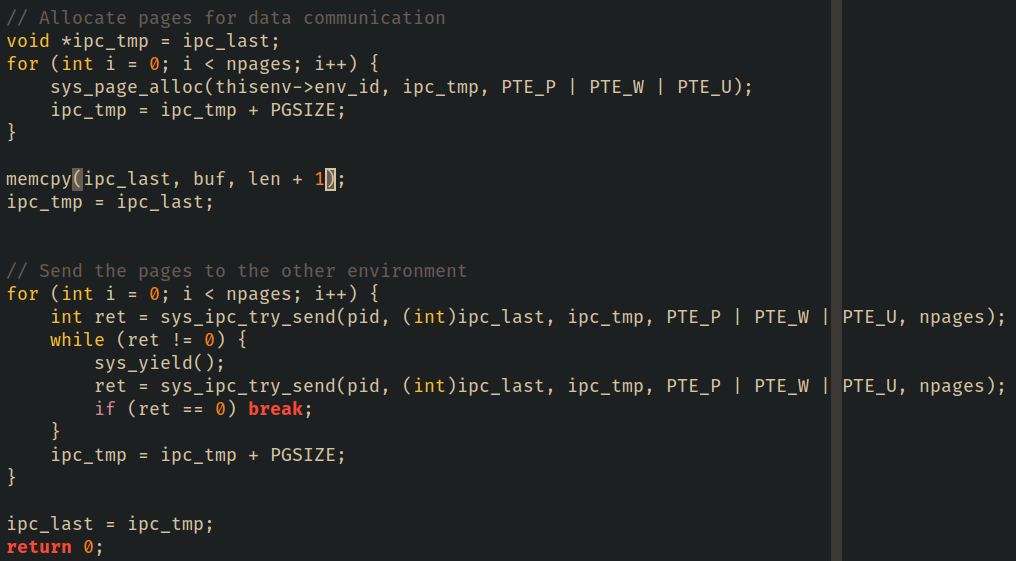
\includegraphics[width=1.0\textwidth]{send2.png}
    \caption{
        ادامه
        متن تابع
        \lr{send\_message}
    }
    \label{fig4output}
\end{figure}
در ادامه به تعدادی که صفحه‌ لازم دارم با استفاده از فراخوانی
\lr{sys\_page\_alloc}
دریافت می‌کنیم.
سپس بافر را در آن صفحات کپی کرده و این صفحات را به پردازه مورد نظر می‌فرستیم. \\
در آخر فراخوانی
\lr{recv\_message}
را داریم که صفحات را دریافت کرده و آدرس اول بافر را به برنامه‌ای که در حال دریافت است بازگشت
می‌دهد.
\begin{figure}[H]
    \centering
    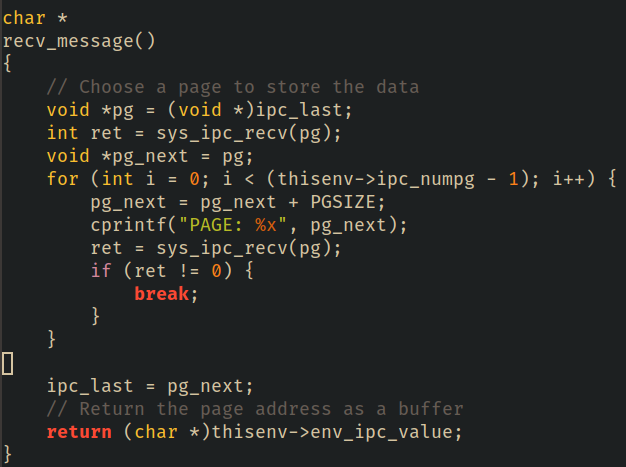
\includegraphics[width=0.8\textwidth]{recv.png}
    \caption{
        متن تابع
        \lr{recv\_message}
    }
    \label{fig5output}
\end{figure}
در این تابع ابتدا تعداد اولین صفحه را دریافت کرده و در محل خودش می‌نوسیم
سپس تعداد صفحه را دریافت کرده و این تعداد صفحه را به ترتیب در جای خودشان می‌نویسیم
و آدرس اول بافر را به برنامه دریافت کننده می‌دهیم. \\
سپس برنامه تست را می‌نوسیم به شرح زیر است.
\begin{figure}[H]
    \centering
    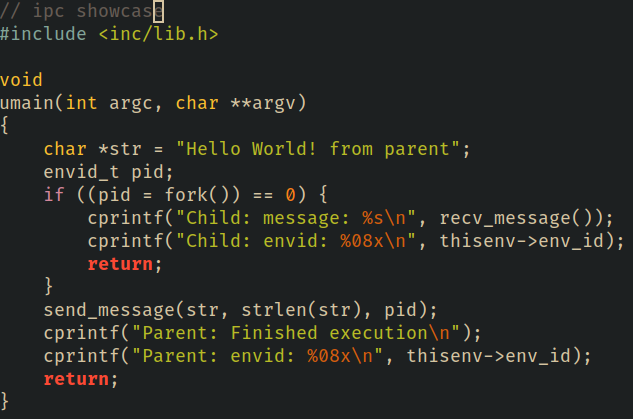
\includegraphics[width=0.8\textwidth]{ipc.png}
    \caption{
        برنامه تست ارتباط میان پردازه‌ای
    }
    \label{fig6output}
\end{figure}
در این برنامه ما یک فراخوانی
\lr{fork}
انجام دادیم. سپس در پردازه فرزند تابع
\lr{recv\_message}
را کال کرده‌ایم که برنامه رو می‌خواباند.
سپس در ادامه والد با صدا زدن
\lr{send\_message}
بافر را برای فرزند می‌فرستد و بافر توسط فرزند چاپ می‌شود.
خروجی سیستم به صورت زیر می‌باشد.
\begin{figure}[H]
    \centering
    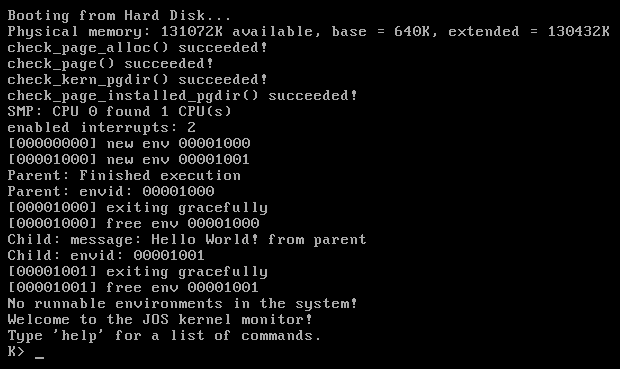
\includegraphics[width=1.0\textwidth]{res.png}
    \caption{
        برنامه تست ارتباط میان پردازه‌ای
    }
    \label{fig7output}
\end{figure}
که در این شکل می‌بینیم که ارتباط به صورت مؤثر برقرار شده است.
\section{نتیجه}
در این تمرین ما با استفاده از پیاده‌سازی های سطح سیستم‌عامل مانند حافظه مجازی و زمان‌بند و بقیه
مواردی که در بالا اشاره کردیم موفق شدیم که ارتباط میان‌ پردازه‌ای را بین دو پردازه فرزند و والد برقرار کنیم.
برقراری این ارتباط توسط حافظه مجازی انجام شد و روش ما به این گونه بود که صفحاتی را در فضای
آدرس فرآیند مورد نظر کپی می‌کردیم تا توسط آن فرآیند مورد استفاده قرار گیرند. \\
کپی کردن صفحه در فرآیند فرزند به صورت
\lr{memcpy}
انجام می‌گرفت. بهتر بود این کار با استفاده از
\lr{Page Fault Handler}
اختصاصی صورت می‌گرفت تا ایده
\lr{CoW}
را نیز پیاده‌سازی کند ولی محض سادگی سراغ این کار رفته نشد.
استفاده از ایده‌هایی که در کرنل
\lr{L3}
مطرح شده است در اینجا به طور کامل ممکن نبود چون که کرنلی که داشتیم نیز به صورت
بسیار ساده بود برای مثال زمان‌بند به صورت پیچیده طراحی نشده است و همچنین پیاده‌سازی
\lr{L3}
بسیار کامل و جامع می‌باشد که پیاده‌سازی آن وقت زیادی می‌برد.
در آخر به جای اینکه در استک پیام‌ها کپی شود به صورت کپی کردن
صفحه انجام می‌شود که در عمل فرق زیادی با کپی کردن پیام در استک ندارد چون که باید
باز هم در این صورت استک که یک پیج است را تغییر دهیم و در موارد واقعی امکان تغییرات
استک برنامه وجود ندارد چون ممکن است دچار
\lr{stack smashing}
شده و برای سیستم باگ‌های امنیتی به وجود بیاوریم.
پس بهتر است از مموری پروتکشن سخت‌افزار استفاده کرده صفحات را کپی کنیم.
در صورتی که سربار کپی صفحات برای ما زیاد است بهتر است ایده
\lr{CoW}
پیاده‌سازی شود.
% \bibliography{references}  % need to put bibtex references in references.bib 
\end{document}
